\documentclass[paper=a4, fontsize=11pt,twoside, abstracton]{scrartcl}
\usepackage[english]{babel}
\usepackage[top=2.5cm, bottom=2.5cm, left=3cm, right=3cm]{geometry}
\newcommand{\SAGAsection}{\small{SAGA}}
\date{\vspace{-5ex}}

% \usepackage[numbers, sort&compress]{natbib}
\usepackage{natbib}           % call natbib
% \setcitestyle{authoryear}     % set citation style to authoryear
\bibliographystyle{plainnat}  % use the plainnat instead of plain


\usepackage{amsmath}
\usepackage{amsthm}
\usepackage{amssymb}
\usepackage{sectsty}
\usepackage{graphicx}
\graphicspath{{./figures/}}
\usepackage{subfigure}
\usepackage{color}
\usepackage{url}
\usepackage{todonotes}
\usepackage{commath}
\usepackage{amsfonts}
\usepackage{mdframed}
\usepackage{enumerate}
\usepackage{bold-extra}
\usepackage{nicefrac}
\usepackage{wrapfig}
\usepackage{caption}
\usepackage{enumitem}

% % For algorithms
\usepackage{algorithm}% http://ctan.org/pkg/algorithms
\usepackage{algpseudocode}% http://ctan.org/pkg/algorithmicx
\usepackage{empheq}


\definecolor{mydarkblue}{rgb}{0,0.08,0.45}
\usepackage[colorlinks=true,
    linkcolor=mydarkblue,
    citecolor=mydarkblue,
    filecolor=mydarkblue,
    urlcolor=mydarkblue,
    pdfview=FitH]{hyperref}

\definecolor{myblue}{HTML}{D2E4FC}
\newcommand*\mybluebox[1]{%
\colorbox{myblue}{\hspace{1em}#1\hspace{1em}}}




\DeclareMathOperator*{\argmin}{arg\,min}
\DeclareMathOperator*{\minimize}{minimize}
\DeclareMathOperator*{\loss}{loss}
\DeclareMathOperator*{\reg}{reg}

\newcommand{\SAGA}{\textsc{Saga}}
\newcommand{\SVRG}{\textsc{Svrg}}
\newcommand{\ProxSVRG}{\textsc{ProxSvrg}}
\newcommand{\blue}{\color{blue}}
\def\RR{{\mathbb R}}
\def\EE{{\mathbb E}}
\def\DD{{\mathcal D}}
\def\prox{{\mathbf{prox}}}
\def\eprox{{\emph{\text{Prox}}}}
\def\xx{{\boldsymbol x}}
\def\uu{{\boldsymbol u}}
\def\ww{{\boldsymbol w}}
\def\yy{{\boldsymbol y}}
\def\vv{{\boldsymbol v}}
\def\hh{{\boldsymbol h}}
\def\ww{{\boldsymbol w}}
\def\WW{{\boldsymbol W}}
\def\zz{{\boldsymbol z}}
\def\bb{{\boldsymbol b}}
\def\ssigma{{\boldsymbol \sigma}}



\newmdtheoremenv{alg}{Algorithm}
\newmdtheoremenv{theo}{Theorem}
\newtheorem{example}{Example}
\newtheorem{theorem}{Theorem}
\newtheorem{lemma}{Lemma}
\newtheorem{proposition}{Proposition}
\newtheorem{remark}{Remark}
\newtheorem{corollary}{Corollary}
\newtheorem{definition}{Definition}
\newtheorem{conjecture}{Conjecture}
\newtheorem{axiom}{Axiom}


\title{Notes on neural networks}
\author{Fabian Pedregosa\thanks{Based on notes and discussion with the NN4Text group at UC Berkeley.}}

\begin{document}
\maketitle



% \section{An algebraic approach to neural networks}

\section{Different types of neural networks}


\paragraph{Notation.} I denote vectors and vector-valued functions in boldface lowercase (e.g. $\xx, \ssigma$) and matrices in uppercase boldface (e.g., $\WW$).

\paragraph{Feed-forward neural networks.} This is the classical and simplest type of deep neural network, made simply by recursively applying a linear transformation followed by a nonlinearity. For a feed-forward neural network with $k$ layers, the output of the model can be characterized by the following recursion for $t=1, \ldots, k$:

\begin{equation}\label{eq:feed_forward}
  \xx_{t} = \ssigma_t(\boldsymbol{W}_{t-1} \xx_{t-1} + \boldsymbol{b}_{t-1}) \,,
\end{equation}
where $\WW_{t}$ are matrices of size $d_{t} \times d_{t-1}$, with $d_0 = $ size of input $\xx_0$, $\boldsymbol{b}_{t-1} \in \RR^{d_t}$ is the vector of bias terms and $\sigma_t: \RR^{d_t} \to  \RR^{d_t}$ is a vector-valued function which often it is separable, but not always, as it might also hold pooling or convolution operations. In many cases, the final prediction is a scalar (e.g., in regression or binary classification), in which case $d_k = 1$ and hence $\WW_k$
is in fact a vector.

\paragraph{Recurrent neural networks.} A recurrent neural network (RNN) is a class of artificial neural network where connections between units form a directed cycle. This creates an internal state of the network which allows it to exhibit dynamic temporal behavior. Unlike feedforward neural networks, RNNs can use their internal memory to process arbitrary sequences of inputs. This makes them applicable to tasks such as unsegmented connected handwriting recognition or speech recognition.

The notation here is slightly different from the previous paragraph. We are \emph{given} a sequence of input vectors $\xx_{t}$, $t=1, \ldots, k$ (note that here the subindex $t$ refers to the order of the sequence and not to the depth of the neural network) and the network computes the sequence of output vectors $\yy_{t}$, $t=1, \ldots, k$ as $$\hh_t = f(\xx_t, \hh_{t-1})$$ where $h_t$ is a hidden state at time $t$.\footnote{These are sometimes referred to as ``context vectors''.}

 For a more precise example of function $f$, consider the Elman network \citep{elman1990finding}. This is expressed as
  \begin{align}
    \hh_{t} &= \sigma_1(\WW_1 \xx_t + \boldsymbol{U}_1 \hh_{t-1} + \boldsymbol{b}_1)  \\
    \yy_t &= \sigma_2(\WW_2\hh_t + \boldsymbol{b}_2)\,,
  \end{align}

The above is a slightly simplified example. In practice, people typically use a slightly more complicated architecture. For example, in \citep{cho2014learning}, the authors use the following architecture for a natural language inference task:
  \begin{align}
    \zz_t &= \sigma(\WW_1 \xx_t + \WW_2 \hh_{t-1} + \bb_1) \\
    \boldsymbol{r}_t &= \sigma(\WW_3 \xx_t + \WW_4 \hh_{t-1} + \bb_2) \\
    \tilde{\hh}_t &= \text{tanh}(\WW_5 \xx_t + \WW_6 (\boldsymbol{r}_t  \odot \hh_{t-1}) + \bb_3) \\
    \hh_t &= (\boldsymbol{1} - \zz_t) \odot \hh_{t-1} + \zz_t \odot\tilde{\hh}_t\,,
  \end{align}
where $\odot$ denotes the element-wise product (Hadamart product to be pendantic) and $\sigma$ is a logistic sigmoid function.

The final state (sometimes called the \emph{decoder} step of a neural network) $\boldsymbol u$ is then computed based on the last states as
\begin{equation}\label{eq:rnn_prediction}
  \uu_t = \text{tanh}(\WW_7 \hh_t + \WW_8 \hh_k + \bb_4) \quad.
\end{equation}
Finally, one predicts a label $\yy_{t}$ from $\uu_t$ with a standard softmax layer.



\paragraph{Attention-augmented recurrent neural networks.} Attention aims to solve the problem of forcing the network to encode all information into one fixed-length vector. Using this mechanism, the network can instead refer back to the input sequence. Personally, I think that attention is somewhat of a misnomer as it is simply giving the network access to its internal memory, which is the hidden state of the encoder. In this interpretation, instead of choosing what to  ``attend'' to, the network chooses what to retrieve from memory. Unlike typical memory, the memory access mechanism here is soft, which means that the network retrieves a weighted combination of all memory locations, not a value from a single discrete location.

In this attention-augmented architecture, the decoding at step $t$ is allowed to see not only the hidden state $\hh_t$ but a weighted sum of these. Each hidden state $\hh_t$ contains information about the whole input sequence with strong focus on the parts surrounding the $T$-th entry (word). Following~\citep{bahdanau2014neural} we define a context vector as a weighted sum of the latent variables $\hh_t$:
\begin{equation}
  \boldsymbol{c}_t = \sum_{j=1}^k \boldsymbol{\alpha}_{jt} \hh_j\,,
\end{equation}
where the weights $\alpha_{i}$ of each latent variable $\hh_j$ sums to one. This is typically computed as the softmax of a vector $\boldsymbol{e}_t$
\begin{equation}
  \boldsymbol{\alpha}_{ij} = \text{softmax}(\boldsymbol{e}_t)\quad, \quad \text{ where } \boldsymbol{e}_{tj} = \boldsymbol{a}(\hh_{t-1}, \hh_j) \quad,
\end{equation}
where $\boldsymbol{a}$ scores how well the inputs around position $j$ and the output at position $t$ match.\footnote{\citet{bahdanau2014neural} considers ``annotations'' and hidden states as two different things while I'm taking them to be the same thing. Is this wrong?} This model $\boldsymbol{a}$ is often parametrized by a feedforward neural network, and jointly trained the rest of the network.



\begin{figure}
  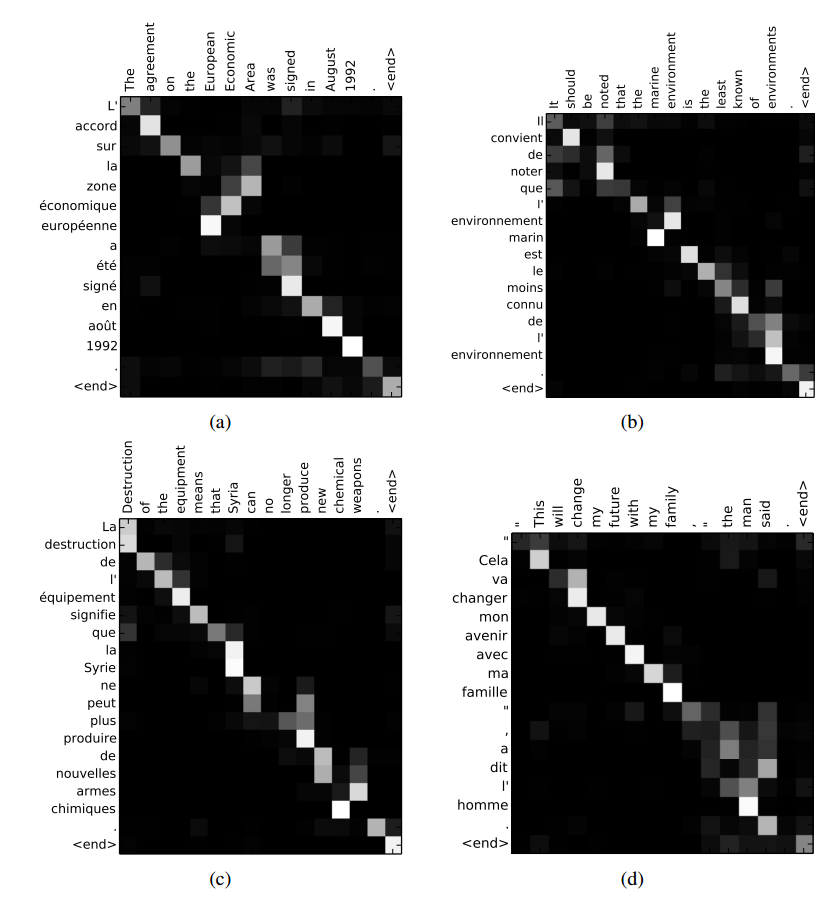
\includegraphics[width=\linewidth]{attention_vis.png}
  \caption{Visualizing the attention weights ($\boldsymbol{\alpha}$) in a translation task.}\label{fig:attention_translation}
\end{figure}

One of the nice side effects of the attention mechanism is that one can inspect  the vector $\boldsymbol{\alpha}$ as a proxy to interpret the decision of an encoder-decoder architecture. See Figure\ref{fig:attention_translation} for an example on a translation task.


\nocite{*}
\bibliography{biblio}{}

\end{document}
